%% LaTeX Beamer presentation template (requires beamer package)
%% see http://bitbucket.org/rivanvx/beamer/wiki/Home
%% idea contributed by H. Turgut Uyar
%% template based on a template by Till Tantau
%% this template is still evolving - it might differ in future releases!

\documentclass{beamer}

\mode<presentation>
{
\usetheme{Warsaw}

\setbeamercovered{transparent}
}

\usepackage[english]{babel}
\usepackage[latin1]{inputenc}

% font definitions, try \usepackage{ae} instead of the following
% three lines if you don't like this look
\usepackage{mathptmx}
\usepackage[scaled=.90]{helvet}
\usepackage{courier}

\usepackage[T1]{fontenc}

% User packages
\usepackage[absolute,overlay]{textpos}
\usepackage{tikz}
\usepackage{listings}

\title{Birdhouse - supporting Web Processing Services}

%\subtitle{}

% - Use the \inst{?} command only if the authors have different
%   affiliation.
\author{\vspace{2.3cm}\\
Carsten Ehbrecht\inst{1}
\and Stephan Kindermann\inst{1}
\and Nils Hempelmann\inst{2}
}
%\author{\inst{1}}

% - Use the \inst command only if there are several affiliations.
% - Keep it simple, no one is interested in your street address.
\institute[Institute]
{
\inst{1}%
DKRZ - German Climate Compute Center
\and
\inst{2}%
GIZ - German Development Cooperation
}

\date{\footnotesize{$28^{th}$ of November 2017/ Python Frameworks Workshop at ECMWF}}


% This is only inserted into the PDF information catalog. Can be left
% out.
\subject{Talks}



% If you have a file called "university-logo-filename.xxx", where xxx
% is a graphic format that can be processed by latex or pdflatex,
% resp., then you can add a logo as follows:

% \pgfdeclareimage[height=0.5cm]{university-logo}{university-logo-filename}
% \logo{\pgfuseimage{university-logo}}



% Delete this, if you do not want the table of contents to pop up at
% the beginning of each subsection:
\AtBeginSubsection[]
{
\begin{frame}<beamer>
\frametitle{Outline}
\tableofcontents[currentsection,currentsubsection]
\end{frame}
}

% Section title slides
\AtBeginSection[]{
  \begin{frame}
  \vfill
  \centering
  \begin{beamercolorbox}[sep=8pt,center,shadow=true,rounded=true]{title}
    \usebeamerfont{title}\insertsectionhead\par%
  \end{beamercolorbox}
  \vfill
  \end{frame}
}


% If you wish to uncover everything in a step-wise fashion, uncomment
% the following command:

%\beamerdefaultoverlayspecification{<+->}

\begin{document}

\begin{frame}
   % \tikz [remember picture,overlay]
   %  \node at
   %      ([yshift=4.8cm]current page.south)
   %      %or: (current page.center)
   %      {
\includegraphics[height=2.8cm]{images/pywps}};
   \titlepage
\end{frame}

\begin{frame}
\frametitle{Outline}
\tableofcontents
% You might wish to add the option [pausesections]
\end{frame}

% %%%%%%%%%%%%%%%%%%%%%%%%%%%%%%%%%%%%%%%%%%%%%%%%%%%%%%%%%%%%%%%%%%%%%%%%%%%%%
\section{Motivation}

%\subsection[Short First Subsection Name]{First Subsection Name}

% -----------------------------------------------
\begin{frame}
\frametitle<presentation>{The OGC Web Processing Service}

\begin{itemize}
\item OGC open web standard for remote geo-spatial processing.
\item Other widley used OGC web standards: \textbf{WMS}, \textbf{WFS}, \textbf{WCS}.
\item Three basic requests:
\begin{itemize}
      \item  \textit{GetCapabilities}
      \item  \textit{DescribeProcess}
      \item  \textit{Execute}
\end{itemize}
\item Three basic input/output classes:
\begin{itemize}
      \item  \textit{Literal}
      \item  \textit{Complex} - for geo-spatial data and services
      \item  \textit{BoundingBox} - for geo-spatial data extent
\end{itemize}
\end{itemize}
\end{frame}

% -----------------------------------------------
\begin{frame}
\frametitle<presentation>{The OGC Web Processing Service}

  \begin{figure}[ht]

   \centering
   
\includegraphics[height=5.85cm]{images/WPS}
  \end{figure}

\centering
\footnotesize{http://www.slideshare.net/TheodorFoerster/restful-web-processing-service}

\end{frame}

% -----------------------------------------------
\begin{frame}
\frametitle<presentation>{WPS Use Case}

  \begin{figure}[ht]
    \centering
    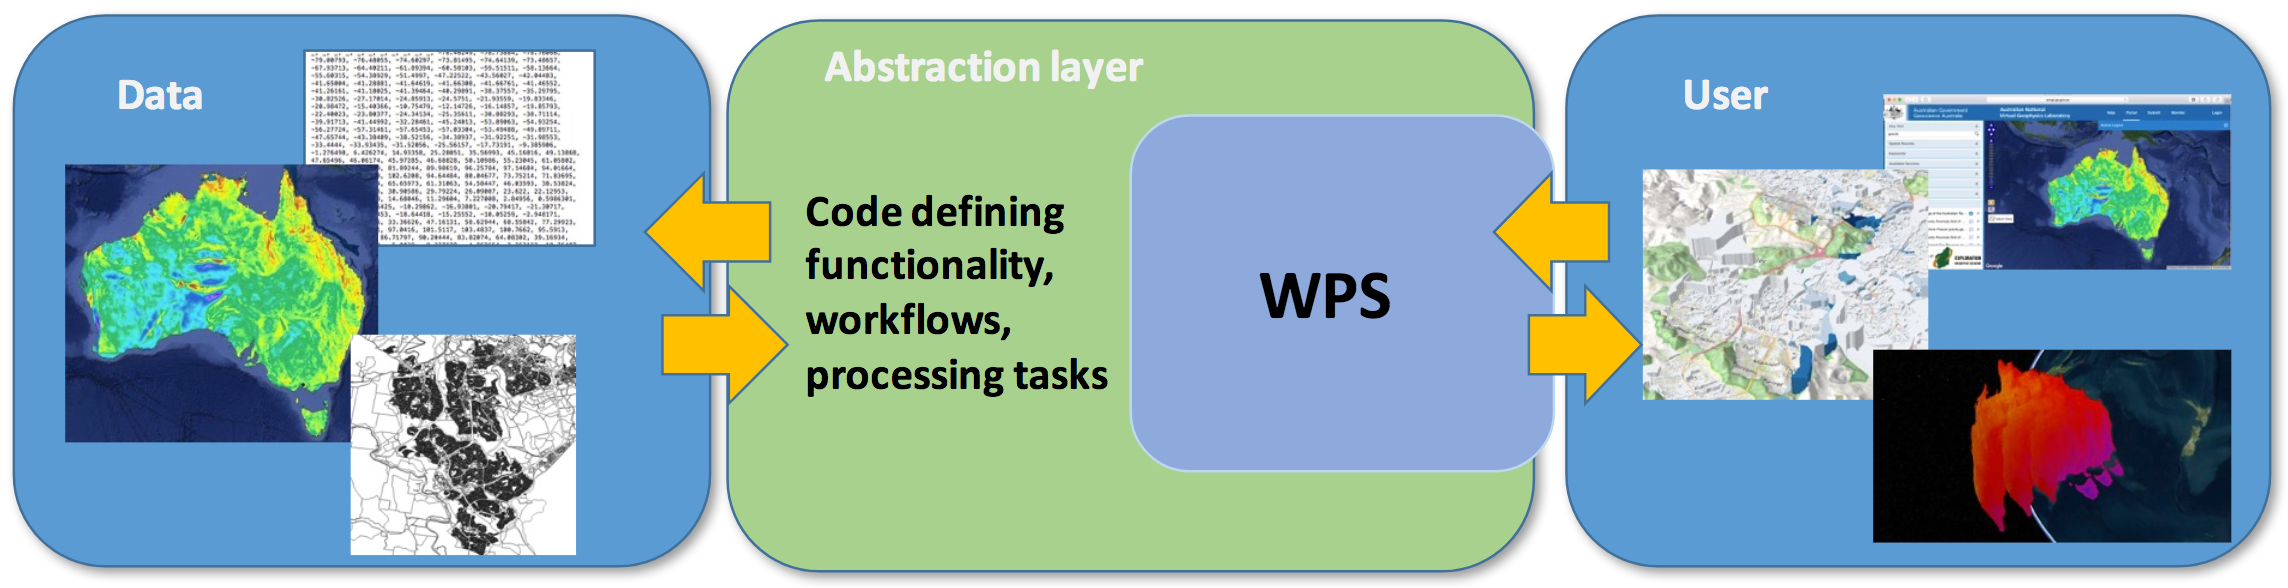
\includegraphics[width=11.5cm]{images/wps_adamsteer}
  \end{figure}

\centering
\footnotesize{WPS for Point Clouds by Adam Steer, NCI, Australia}

\end{frame}

% -----------------------------------------------
\begin{frame}
\frametitle<presentation>{WPS Inputs and Outputs}

  \begin{figure}[ht]
    \centering
    \includegraphics[width=11.5cm]{images/wps-ensemble-robustness}
  \end{figure}

\end{frame}

% -----------------------------------------------
\begin{frame}
  \frametitle<presentation>{What does WPS provide?}
  \begin{itemize}
    \item web access to your algorithms (GET request with key-value, POST request with xml)
    \item WPS knows about the inputs and outpus of a process
    \item processes are self-describing (GetCapabilites, DescribeProcess)
    \item sync and async calls (async calls with status document)
    \item its a standard interface ... several implementations are available (PyWPS, GeoServer, 52 North, COWS, ...)
    \item process definition is easy to write
    \item not restricted to a specific programming language
    \item can be used internally to provide enhanced functionality to web portals
  \end{itemize}
\end{frame}

% -----------------------------------------------
\begin{frame}[fragile]
  \frametitle<presentation>{Enable your code as WPS process}
  \begin{block}{Use wps decorator for your function}
    \tiny
    \lstset{language=python}
    \lstinputlisting{static/wps_myplot.py}
  \end{block}
  \begin{block}{Execute your function with WPS}
    \begin{verbatim}
http://localhost/wps?service=WPS&version=1.0.0 \
 &request=execute \
 &identifier=myplot \
 &DataInputs=nc_file=http://;variable=tas
    \end{verbatim}
  \end{block}
\end{frame}

% %%%%%%%%%%%%%%%%%%%%%%%%%%%%%%%%%%%%%%%%%%%%%%%%%%%%%%%%%%%%%%%%%%%%%%%%%%%%%
\section{PyWPS}

% -----------------------------------------------
\begin{frame}
\frametitle{What is PyWPS?}

\begin{itemize}
  \item An implementation of the OGC Web Processing Service standard
  \item Coded on the Python language (researcher friendly)
  \item Started in the Spring of 2006
  \item Relevant contributions by over a dozen individuals
  \item New licence: MIT
  \item OSGeo accreditation around the corner \ldots
  \item http://pywps.org

\end{itemize}
\end{frame}

% -----------------------------------------------
\begin{frame}
\frametitle{What is PyWPS good for?}

\begin{itemize}
  \item Make your models available to the world
  \item Enables remote processing of complex and/or lengthy models
  \item Guarantees model inputs fit basic requirements
        (e.g. type, number)
  \item Guarantees interoperability of model inputs and outputs
  \begin{itemize}
    \item using the OGC data standards
	\item formalizing input/output data types
  \end{itemize}
\end{itemize}
\end{frame}

% -----------------------------------------------
\begin{frame}
\frametitle<presentation>{The role of a WSGI server}

\begin{itemize}
  \item WSGI - Common interface to multiple web applications frameworks
  \item WSGI Server - basic functions:
  \begin{itemize}
    \item accepts HTTP requests
    \item replies to HTTP requests
  \end{itemize}
  \item WSGI provides \textit{concurrency}, allowing multiple:
  \begin{itemize}
    \item threads
    \item workers
    \item processes
  \end{itemize}
\end{itemize}
\end{frame}

% -----------------------------------------------
\begin{frame}
\frametitle<presentation>{Gunicorn (Green Unicorn)}

\begin{tikzpicture}[remember picture,overlay]
    \node[xshift=-2.5cm,yshift=-4cm] at (current page.north east)
    {\includegraphics[height=2.2cm]{images/GUnicorn}};
\end{tikzpicture}

\begin{itemize}
  \item It is one of many WSGI servers out there
  \item Easy to configure and use with Python
  \item Promotes the concepts of ``workers''
  \begin{itemize} \item essentially OS processes \end{itemize}
  \item Each worker can run on a different CPU core
  \begin{itemize} \item a worker can be a Flask application instance
  \end{itemize}
\end{itemize}

\centering
\footnotesize{http://gunicorn.org}

\end{frame}

% -----------------------------------------------
\begin{frame}
\frametitle<presentation>{Nginx}

\begin{tikzpicture}[remember picture,overlay]
    \node[xshift=-2.6cm,yshift=-3.4cm] at (current page.north east)
    {
\includegraphics[height=0.8cm]{images/nginx}};
\end{tikzpicture}

\begin{itemize}
  \item Essentially a web (HTTP) server
  \item But more used for reverse-proxy
  \item Acts as a single entrance point to all requests
  \item Redirects requests to Gunicorn
  \item Can redirect to multiple Gunicorns
  \item Gateway to multiple servers and applications from a single URL
\end{itemize}

\centering
\footnotesize{http://nginx.org/}

\end{frame}

% -----------------------------------------------
\begin{frame}
\frametitle<presentation>{The WSGI Onion}

\begin{tikzpicture}[remember picture,overlay]
    \node[xshift=-9.2cm,yshift=-5.8cm] at (current page.north east)
    {\includegraphics[height=6cm]{images/OnionWSGI_all}};
\end{tikzpicture}

\begin{textblock*}{5cm}(7cm,4cm)
\begin{itemize}
  \item Nginx - security, reverse proxy, load balancing
  \item Gunicorn - concurrency, WSGI
  \item Flask - web application framework
\end{itemize}
\end{textblock*}
\end{frame}


% -----------------------------------------------
\begin{frame}
\frametitle<presentation>{It's complicated!}

\begin{itemize}

  \item Scalability requires the orchestration of various software layers:
   \begin{itemize}
	  \item Nginx
	  \item Gunicorn
	  \item Flask
	  \item PyWPS
	\end{itemize}
  \item Many packages to install
  \item Many configurations to set-up
\end{itemize}

\vspace{0.4cm}
\centering
\Large{Too much work?}

\end{frame}

% -----------------------------------------------
\begin{frame}
\frametitle<presentation>{Advanced: PyWPS Scheduler Extension}

  \begin{figure}[ht]
    \centering
    \includegraphics[width=11.5cm]{images/pywps-scheduler-extension}
  \end{figure}

  \centering
  \footnotesize{This extension is used by the CP4CDS Copernicus project}

\end{frame}


% %%%%%%%%%%%%%%%%%%%%%%%%%%%%%%%%%%%%%%%%%%%%%%%%%%%%%%%%%%%%%%%%%%%%%%%%%%%%%
\section{Birdhouse}

% -----------------------------------------------
\begin{frame}
\frametitle<presentation>{What is Birdhouse?}

\begin{itemize}
  \item Supporting OGC Web Processing Services in the climate science community.
  \item Making it easier to setup WPS services (Birdhouse-Builder).
  \item Providing Python library and WPS processes to access climate data.
  \item Providing a workflow to chain data fetching and data processing.
  \item Providing a web and command line client to interact with WPS services.
  \item http://bird-house.github.io/

\end{itemize}
\end{frame}


% -----------------------------------------------
\begin{frame}
\frametitle<presentation>{Birdhouse Overview}

  \begin{figure}[ht]
    \centering
    \includegraphics[height=5.85cm]{images/birdhouse-overview}
  \end{figure}

\end{frame}

% -----------------------------------------------
\begin{frame}
\frametitle<presentation>{WSGI Application controlled by Supervisor}

  \begin{figure}[ht]
    \centering
    \includegraphics[height=5.85cm]{images/wsgi-app}
  \end{figure}

\end{frame}

% -----------------------------------------------
\begin{frame}
  \frametitle<presentation>{Phoenix web-based WPS client}
  \begin{figure}
    \includegraphics[width=11.5cm]{images/phoenix.png}
  \end{figure}
\end{frame}

% -----------------------------------------------
\begin{frame}[fragile]
  \frametitle<presentation>{Birdy command line WPS client}
  \begin{verbatim}
>> conda install -c birdhouse birdhouse-birdy
>> export WPS_SERVICS=http://localhost:8094/wps
>> birdy -h
  \end{verbatim}
  \begin{figure}
    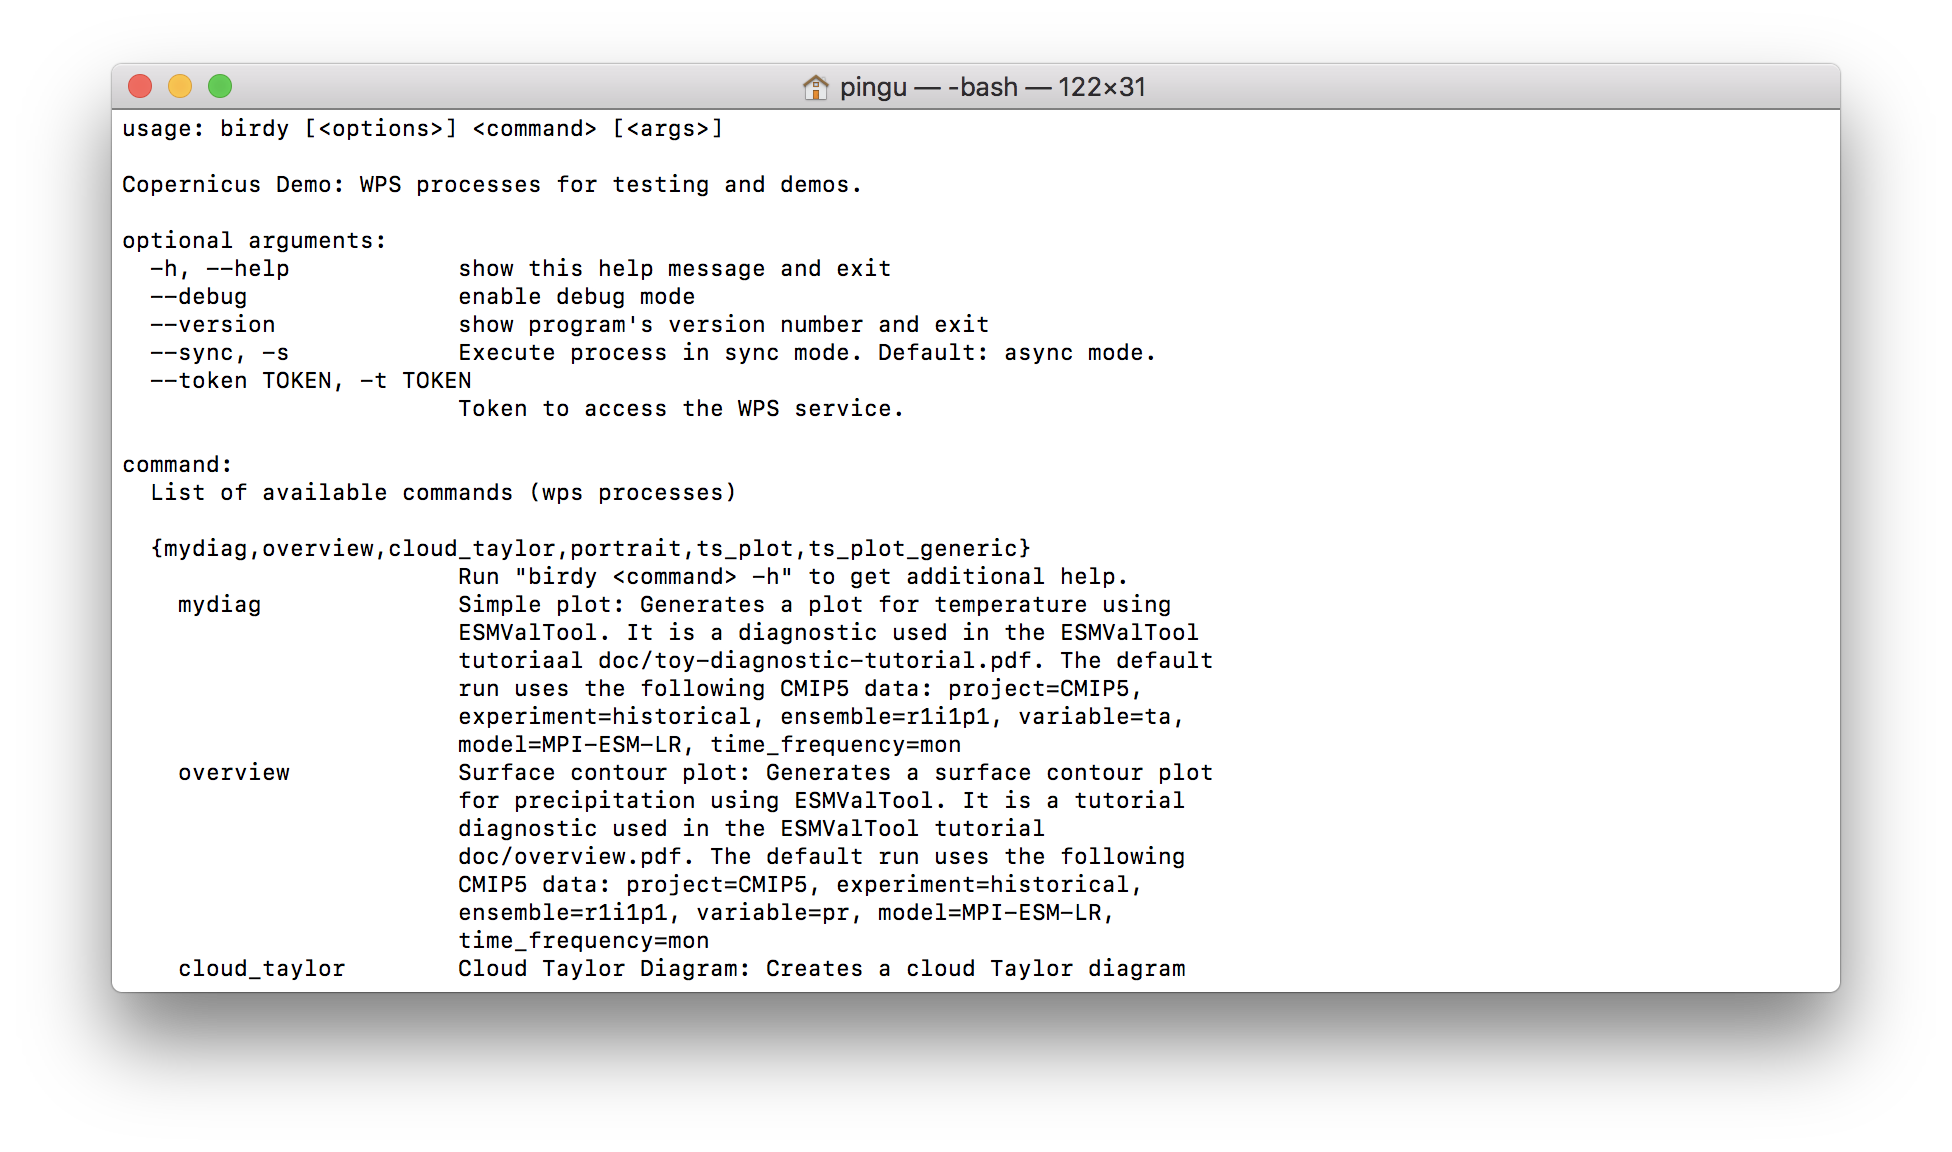
\includegraphics[width=11.5cm]{images/birdy-terminal}
  \end{figure}
\end{frame}

% -----------------------------------------------
\begin{frame}
  \frametitle<presentation>{Why Conda and Buildout?}
  \begin{itemize}
    \item many components: WPS, WMS, web-server, solr, ...
    \item lots of dependencies: cdo, cfchecker, ocgis, numpy, R, ...
    \item many different kinds of config files need to be configured
    \item installation needs to be reproducible at different locations
    \item should work with different Linux distributions (Centos, Fedora, Debian, Ubuntu, ...)
  \end{itemize}
  \begin{figure}
    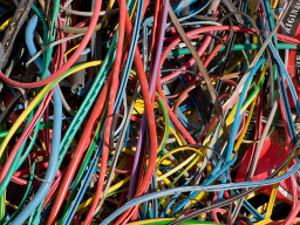
\includegraphics[width=4cm]{images/chaos}
  \end{figure}
\end{frame}

% -----------------------------------------------
\begin{frame}[fragile]
  \frametitle<presentation>{Conda Package Manager}
  \begin{itemize}
    \item originally for python ... but has a general concept
    \item does not need admin rights
    \item manages dependencies
  \end{itemize}
  \begin{block}{install from birdhouse channel}
    \begin{verbatim}
>> conda install -c birdhouse pywps cdo
    \end{verbatim}
  \end{block}
  \begin{block}{create conda environment=emu}
    \begin{verbatim}
>> conda create -n emu -c birdhouse \
      python=2.7 cdo pywps
    \end{verbatim}
  \end{block}
\end{frame}

% -----------------------------------------------
\begin{frame}
  \frametitle<presentation>{Buildout}
  \begin{itemize}
    \item Python based build system
    \item creates application with multiple components including configuration files
    \item works also for non-Python parts
    \item using a buildout configuration
    \item can be extended with recipes
  \end{itemize}
\end{frame}

% -----------------------------------------------
\begin{frame}[fragile]
  \frametitle<presentation>{Install Birdhouse Component with Buildout}
  \begin{itemize}
    \item for convienience there is a Makefile to call the buildout commands
    \item all Birdhouse components (WPS, Phoenix) are installed in the same way
  \end{itemize}
  \begin{block}{First installation}
    \begin{verbatim}
>> git clone https://github.com/bird-house/emu.git
>> cd emu
>> make clean install
>> make start
    \end{verbatim}
  \end{block}
\begin{block}{Update configuration like hostname, port}
    \begin{verbatim}
>> vim custom.cfg
>> make update
>> make restart
    \end{verbatim}
  \end{block}
\end{frame}

% -----------------------------------------------
\begin{frame}
\frametitle<presentation>{Docker}

\begin{tikzpicture}[remember picture,overlay]
    \node[xshift=-3cm,yshift=-5cm] at (current page.north east)
    {\includegraphics[height=4cm]{images/docker}};
\end{tikzpicture}

\begin{itemize}
  \item An OS level virtualisation engine
  \item Docker runs software \textit{containers}
  \begin{itemize} \item a very light weight virtual machine \end{itemize}
  \item Uses Linux kernel namespaces to isolate\\ available resources:
  \begin{itemize}
    \item operating environment
    \item process and user IDs
    \item process trees
    \item network
	\item mounted file systems
  \end{itemize}
  \item Virtualisation provided by the OS itself
\end{itemize}

\centering
\footnotesize{https://docker.com}

\end{frame}

% -----------------------------------------------
\begin{frame}[fragile,shrink]
  \frametitle<presentation>{Try a Docker ...}
  \begin{block}{Images are available on DockerHub}
    \url{https://hub.docker.com/u/birdhouse/}
  \end{block}
  \begin{block}{Start a docker image with Emu WPS}
    \begin{verbatim}
>> docker run -it -p 8090:8090 -p 8094:8094 \
       --name=emu_wps birdhouse/emu
    \end{verbatim}
  \end{block}
  \begin{block}{Run WPS GetCapabilities Request}
    \begin{verbatim}
http://localhost:8094/wps? \
 service=WPS&version=1.0.0&request=getcapabilities
    \end{verbatim}
  \end{block}
\end{frame}

% -----------------------------------------------
\begin{frame}
  \frametitle{WPS Security Proxy}
  \begin{itemize}
    \item using string token (uuid) as part of URL or in request header to protect WPS execute access
    \item X509 certificates to access (remote) data from ESGF are provided by proxy (using environ)
    \item implemented as WSGI application layer
  \end{itemize}
  \begin{figure}
    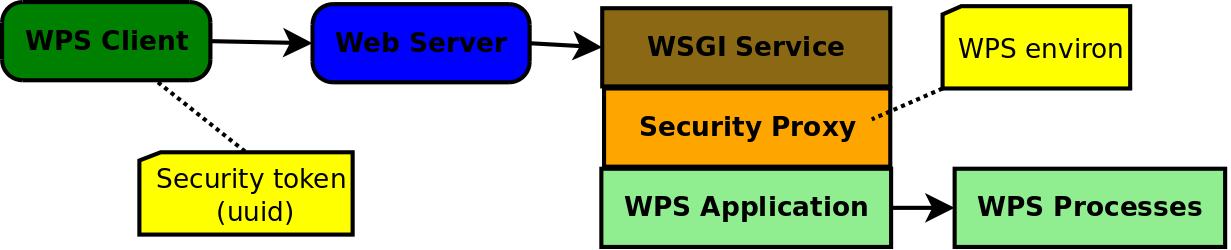
\includegraphics[width=11.5cm]{images/wps-proxy}
  \end{figure}
\end{frame}

% -----------------------------------------------
\begin{frame}
\frametitle<presentation>{Twitcher Security Proxy}

  \begin{figure}[ht]
    \centering
    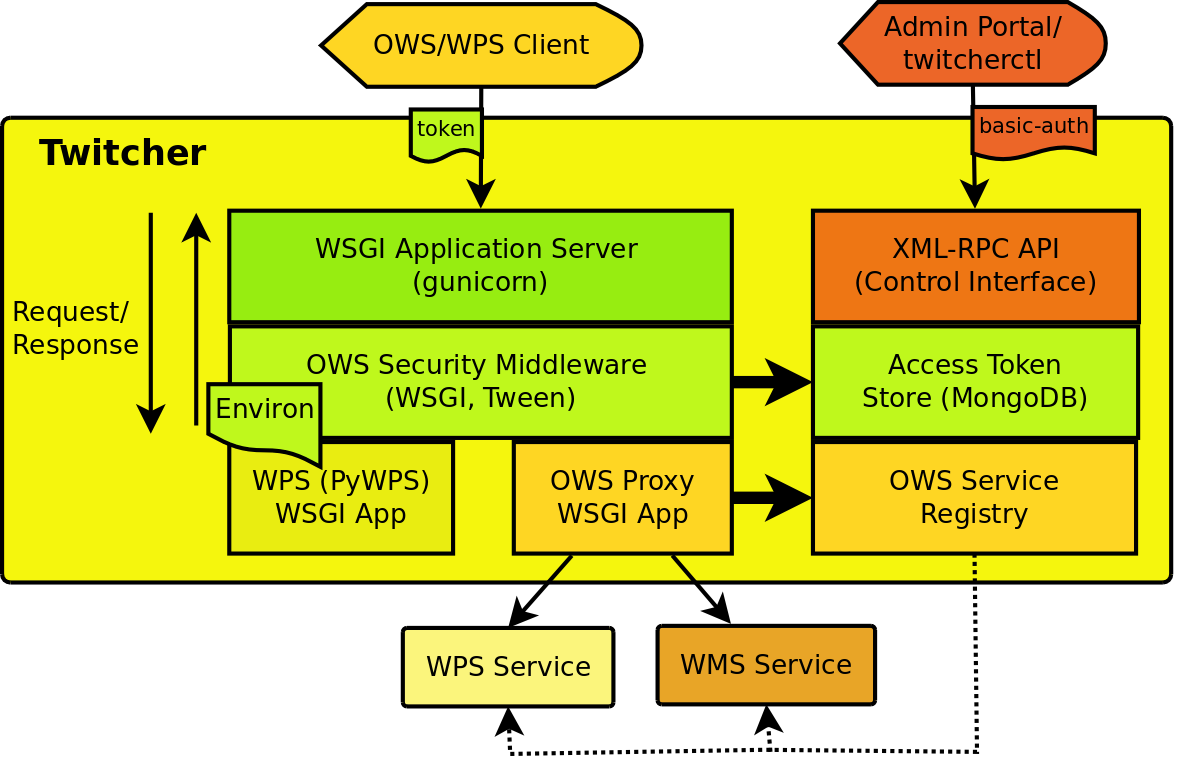
\includegraphics[height=5.85cm]{images/twitcher}
  \end{figure}

\end{frame}


% %%%%%%%%%%%%%%%%%%%%%%%%%%%%%%%%%%%%%%%%%%%%%%%%%%%%%%%%%%%%%%%%%%%%%%%%%%%%%
\section{Summary}

\begin{frame}
\frametitle<presentation>{Summary}

\begin{itemize}

  \item Deployment
  \begin{itemize}
    \item Nginx + Gunicorn provide the infrastructure for scalable services
    \item Scalability implies increased complexity
  \end{itemize}

  \item{Docker containers}
  \begin{itemize}
    \item dockerfiles create pre-configured PyWPS images
    \item set up and deployment complexity already in place
  \end{itemize}

  \item{Get your hands dirty}
  \begin{itemize}
    \item Birdhouse Workshop: \url{http://birdhouse-workshop.readthedocs.io/en/latest/index.html}
    \item PyWPS Workshop: \url{https://github.com/PyWPS/pywps-workshop}
  \end{itemize}
\end{itemize}

\end{frame}

% --------------------------------------------------------------
\begin{frame}
%\frametitle<presentation>{}

  \begin{figure}[ht]
   \centering
   
\includegraphics[height=3cm]{images/pywps}
  \end{figure}

\centering
\Huge{Thank you!}

\vspace{0.4cm}
\normalsize{http://bird-house.github.io/}
\end{frame}

\end{document}
